\documentclass[a4paper,11pt]{jsarticle}

% 数式
\usepackage{amsmath,amsfonts}
\usepackage{amsthm}
\usepackage{bm}
\usepackage{mathtools}
\usepackage{amssymb}

% 表
\usepackage[utf8]{inputenc}
\usepackage{diagbox} % 斜線付きセルを作成するために必要
\usepackage{booktabs} % 表の罫線を美しくするために必要
\usepackage{hhline} % 水平罫線を制御するために必要

% 画像
\usepackage[dvipdfmx]{graphicx}
\usepackage{ascmac}
\usepackage{physics}
\usepackage{float} % 追加

% 図
\usepackage[dvipdfmx]{graphicx}
\usepackage{tikz} %図を描く
\usetikzlibrary{positioning, intersections, calc, arrows.meta,math} %tikzのlibrary

% ハイパーリンク
\usepackage[dvipdfm,
  colorlinks=false,
  bookmarks=true,
  bookmarksnumbered=false,
  pdfborder={0 0 0},
  bookmarkstype=toc]{hyperref}

% 式番号を章ごとにリセット
\numberwithin{equation}{section}

\begin{document}

\title{二体問題で楽をしよう}
\maketitle

\section{はじめに}
このノートは、大学受験の物理における二体問題において、時短する方法をまとめたものである。

\section{よく使う公式}
二物体の質量をそれぞれ$m_1$、$m_2$、速度をそれぞれ$v_1$、$v_2$とする。

\subsection{重心速度}
二体の重心速度は、
\begin{align}
    v_{\text{g}} = \frac{m_1v_1 + m_2v_2}{m_1 + m_2}
\end{align}
により定義される。

二体の重心速度は、外力が働かない限り一定であることが知られている。それぞれの物体について運動方程式を考えると、
\begin{align}
    m_1a_1 &= F_{\text{1}} + f_{21} \\
    m_2a_2 &= F_{\text{2}} + f_{12}
\end{align}
となる。ただし、$f_{21}$は物体1が物体2に受ける力であり、$f_{12}$は物体2が物体1に受ける力である。また、$F_{\text{1}}$は物体1に働く外力であり、$F_{\text{2}}$は物体2に働く外力である。両辺足し合わせると、
\begin{align}
        m_1a_1 + m_2a_2 = F_{\text{1}} + F_{\text{2}}
\end{align}
となる。ただし、作用反作用の法則より、$f_{21} + f_{12} = 0$であることを用いた。次に、両辺$1 = \frac{m_1 + m_2}{m_1 + m_2}$をかけると、
\begin{align}
        (m_1 + m_2)\frac{m_1a_1 + m_2a_2}{m_1 + m_2} = F_{\text{1}} + F_{\text{2}}
\end{align}
となる。したがって、
\begin{align}
        Ma_{\text{g}} = F_{\text{1}} + F_{\text{2}}
\end{align}
となる。ただし、
\begin{align}
        a_{\text{g}} &= \frac{m_1a_1 + m_2a_2}{m_1 + m_2} \quad :\text{重心加速度} \\
        M &= m_1 + m_2 \quad :\text{全質量}
\end{align}
である。ところで、全系に外力が働かない限り、$F_{\text{1}} + F_{\text{2}} = 0$である。したがって、
\begin{align}
    Ma_{\text{g}} = 0
\end{align}
となる。したがって、$a_{\text{g}} = 0$であるから、
\begin{align}
    v_{\text{g}} = \text{一定}
\end{align}
である。したがって、外力が働かない限り二体の重心速度は一定である。

\subsection{運動エネルギー}
二体の運動エネルギーは、
\begin{align}
    K = \frac{1}{2}m_1v_1^2 + \frac{1}{2}m_2v_2^2
\end{align}
であった。これは、重心速度および相対速度を用いて、
\begin{align}
    K = \frac{1}{2}Mv_{\text{g}}^2 + \frac{1}{2}\mu v_{\text{r}}^2
\end{align}
と書き換えることができる。ただし、
\begin{align}
    v_{\text{g}} &= \frac{m_1v_1 + m_2v_2}{m_1 + m_2}\quad : \text{重心速度} \\
    v_{\text{r}} &= v_1 - v_2\quad : \text{相対速度} \\
    M &= m_1 + m_2 \quad: \text{全質量} \\
    \mu &= \frac{m_1m_2}{m_1 + m_2} \quad: \text{換算質量}
\end{align}
である。

\textbf{Prf.}\\
まず、二体の運動エネルギーを次のように書く。
\begin{align}
    K = \frac{1}{2}m_1v_1^2 + \frac{1}{2}m_2v_2^2
\end{align}
次に、$v_1$と$v_2$を重心速度$v_{\text{g}}$と相対速度$v_{\text{r}}$を用いて表す。
\begin{align}
    v_1 &= v_{\text{g}} + \frac{m_2}{M}v_{\text{r}} \\
    v_2 &= v_{\text{g}} - \frac{m_1}{M}v_{\text{r}}
\end{align}
これを運動エネルギーの式に代入する。
\begin{align}
    K &= \frac{1}{2}m_1\left(v_{\text{g}} + \frac{m_2}{M}v_{\text{r}}\right)^2 + \frac{1}{2}m_2\left(v_{\text{g}} - \frac{m_1}{M}v_{\text{r}}\right)^2 \\
    &= \frac{1}{2}m_1\left(v_{\text{g}}^2 + 2v_{\text{g}}\frac{m_2}{M}v_{\text{r}} + \left(\frac{m_2}{M}v_{\text{r}}\right)^2\right) + \frac{1}{2}m_2\left(v_{\text{g}}^2 - 2v_{\text{g}}\frac{m_1}{M}v_{\text{r}} + \left(\frac{m_1}{M}v_{\text{r}}\right)^2\right) \\
    &= \frac{1}{2}m_1v_{\text{g}}^2 + m_1v_{\text{g}}\frac{m_2}{M}v_{\text{r}} + \frac{1}{2}m_1\left(\frac{m_2}{M}v_{\text{r}}\right)^2 + \frac{1}{2}m_2v_{\text{g}}^2 - m_2v_{\text{g}}\frac{m_1}{M}v_{\text{r}} + \frac{1}{2}m_2\left(\frac{m_1}{M}v_{\text{r}}\right)^2
\end{align}
ここで、$m_1v_{\text{g}}\frac{m_2}{M}v_{\text{r}}$と$-m_2v_{\text{g}}\frac{m_1}{M}v_{\text{r}}$は打ち消し合うので、
\begin{align}
    K &= \frac{1}{2}m_1v_{\text{g}}^2 + \frac{1}{2}m_2v_{\text{g}}^2 + \frac{1}{2}m_1\left(\frac{m_2}{M}v_{\text{r}}\right)^2 + \frac{1}{2}m_2\left(\frac{m_1}{M}v_{\text{r}}\right)^2 \\
    &= \frac{1}{2}(m_1 + m_2)v_{\text{g}}^2 + \frac{1}{2}m_1\frac{m_2^2}{M^2}v_{\text{r}}^2 + \frac{1}{2}m_2\frac{m_1^2}{M^2}v_{\text{r}}^2 \\
    &= \frac{1}{2}Mv_{\text{g}}^2 + \frac{1}{2}\left(\frac{m_1m_2^2 + m_2m_1^2}{M^2}\right)v_{\text{r}}^2 \\
    &= \frac{1}{2}Mv_{\text{g}}^2 + \frac{1}{2}\left(\frac{m_1m_2(m_1 + m_2)}{M^2}\right)v_{\text{r}}^2 \\
    &= \frac{1}{2}Mv_{\text{g}}^2 + \frac{1}{2}\left(\frac{m_1m_2}{M}\right)v_{\text{r}}^2 \\
    &= \frac{1}{2}Mv_{\text{g}}^2 + \frac{1}{2}\mu v_{\text{r}}^2
\end{align}
したがって、二体の運動エネルギーは重心速度および相対速度を用いて次のように表される。
\begin{align}
    K = \frac{1}{2}Mv_{\text{g}}^2 + \frac{1}{2}\mu v_{\text{r}}^2
\end{align}
\qed\\

\subsection{反発係数}
高校の教科書において、反発係数は次のように定義されているようである。
\begin{align}
    e = -\frac{v_2' - v_1'}{v_2 - v_1}
\end{align}
ただし、$v_1$は物体1の衝突前の速度、$v_2$は物体2の衝突前の速度、$v_1'$は物体1の衝突後の速度、$v_2'$は物体2の衝突後の速度である。\\
しかし、以下のようにした方が計算が楽である。
\begin{align}
    v_1' - v_{\text{g}} &= -e(v_1 - v_{\text{g}}) \label{collision1} \\
    v_2' - v_{\text{g}} &= -e(v_2 - v_{\text{g}}) \label{collision2}
\end{align}
ただし、$v_{\text{g}}$は重心速度である。定義が等価なことを示す。

\textbf{Prf.}\\
式(\ref{collision2})から式(\ref{collision1})を引くと、
\begin{align}
    v_2' - v_1' &= -e(v_2 - v_{\text{g}}) + e(v_1 - v_{\text{g}})\\
    &= -e(v_2 - v_1)
\end{align}
となる。したがって、定義が等価であることが示された。\\

\section{応用例}
以上の公式を使うと、以下のような問題が3分もあれば解けるようになる。\\
\textbf{問題}\\
以下のような、物体1と物体2が質量$m_1$および$m_2$で、物体2の斜面部分を1が登っていくような問題を考える。
\begin{figure}[H]
    \begin{center}
    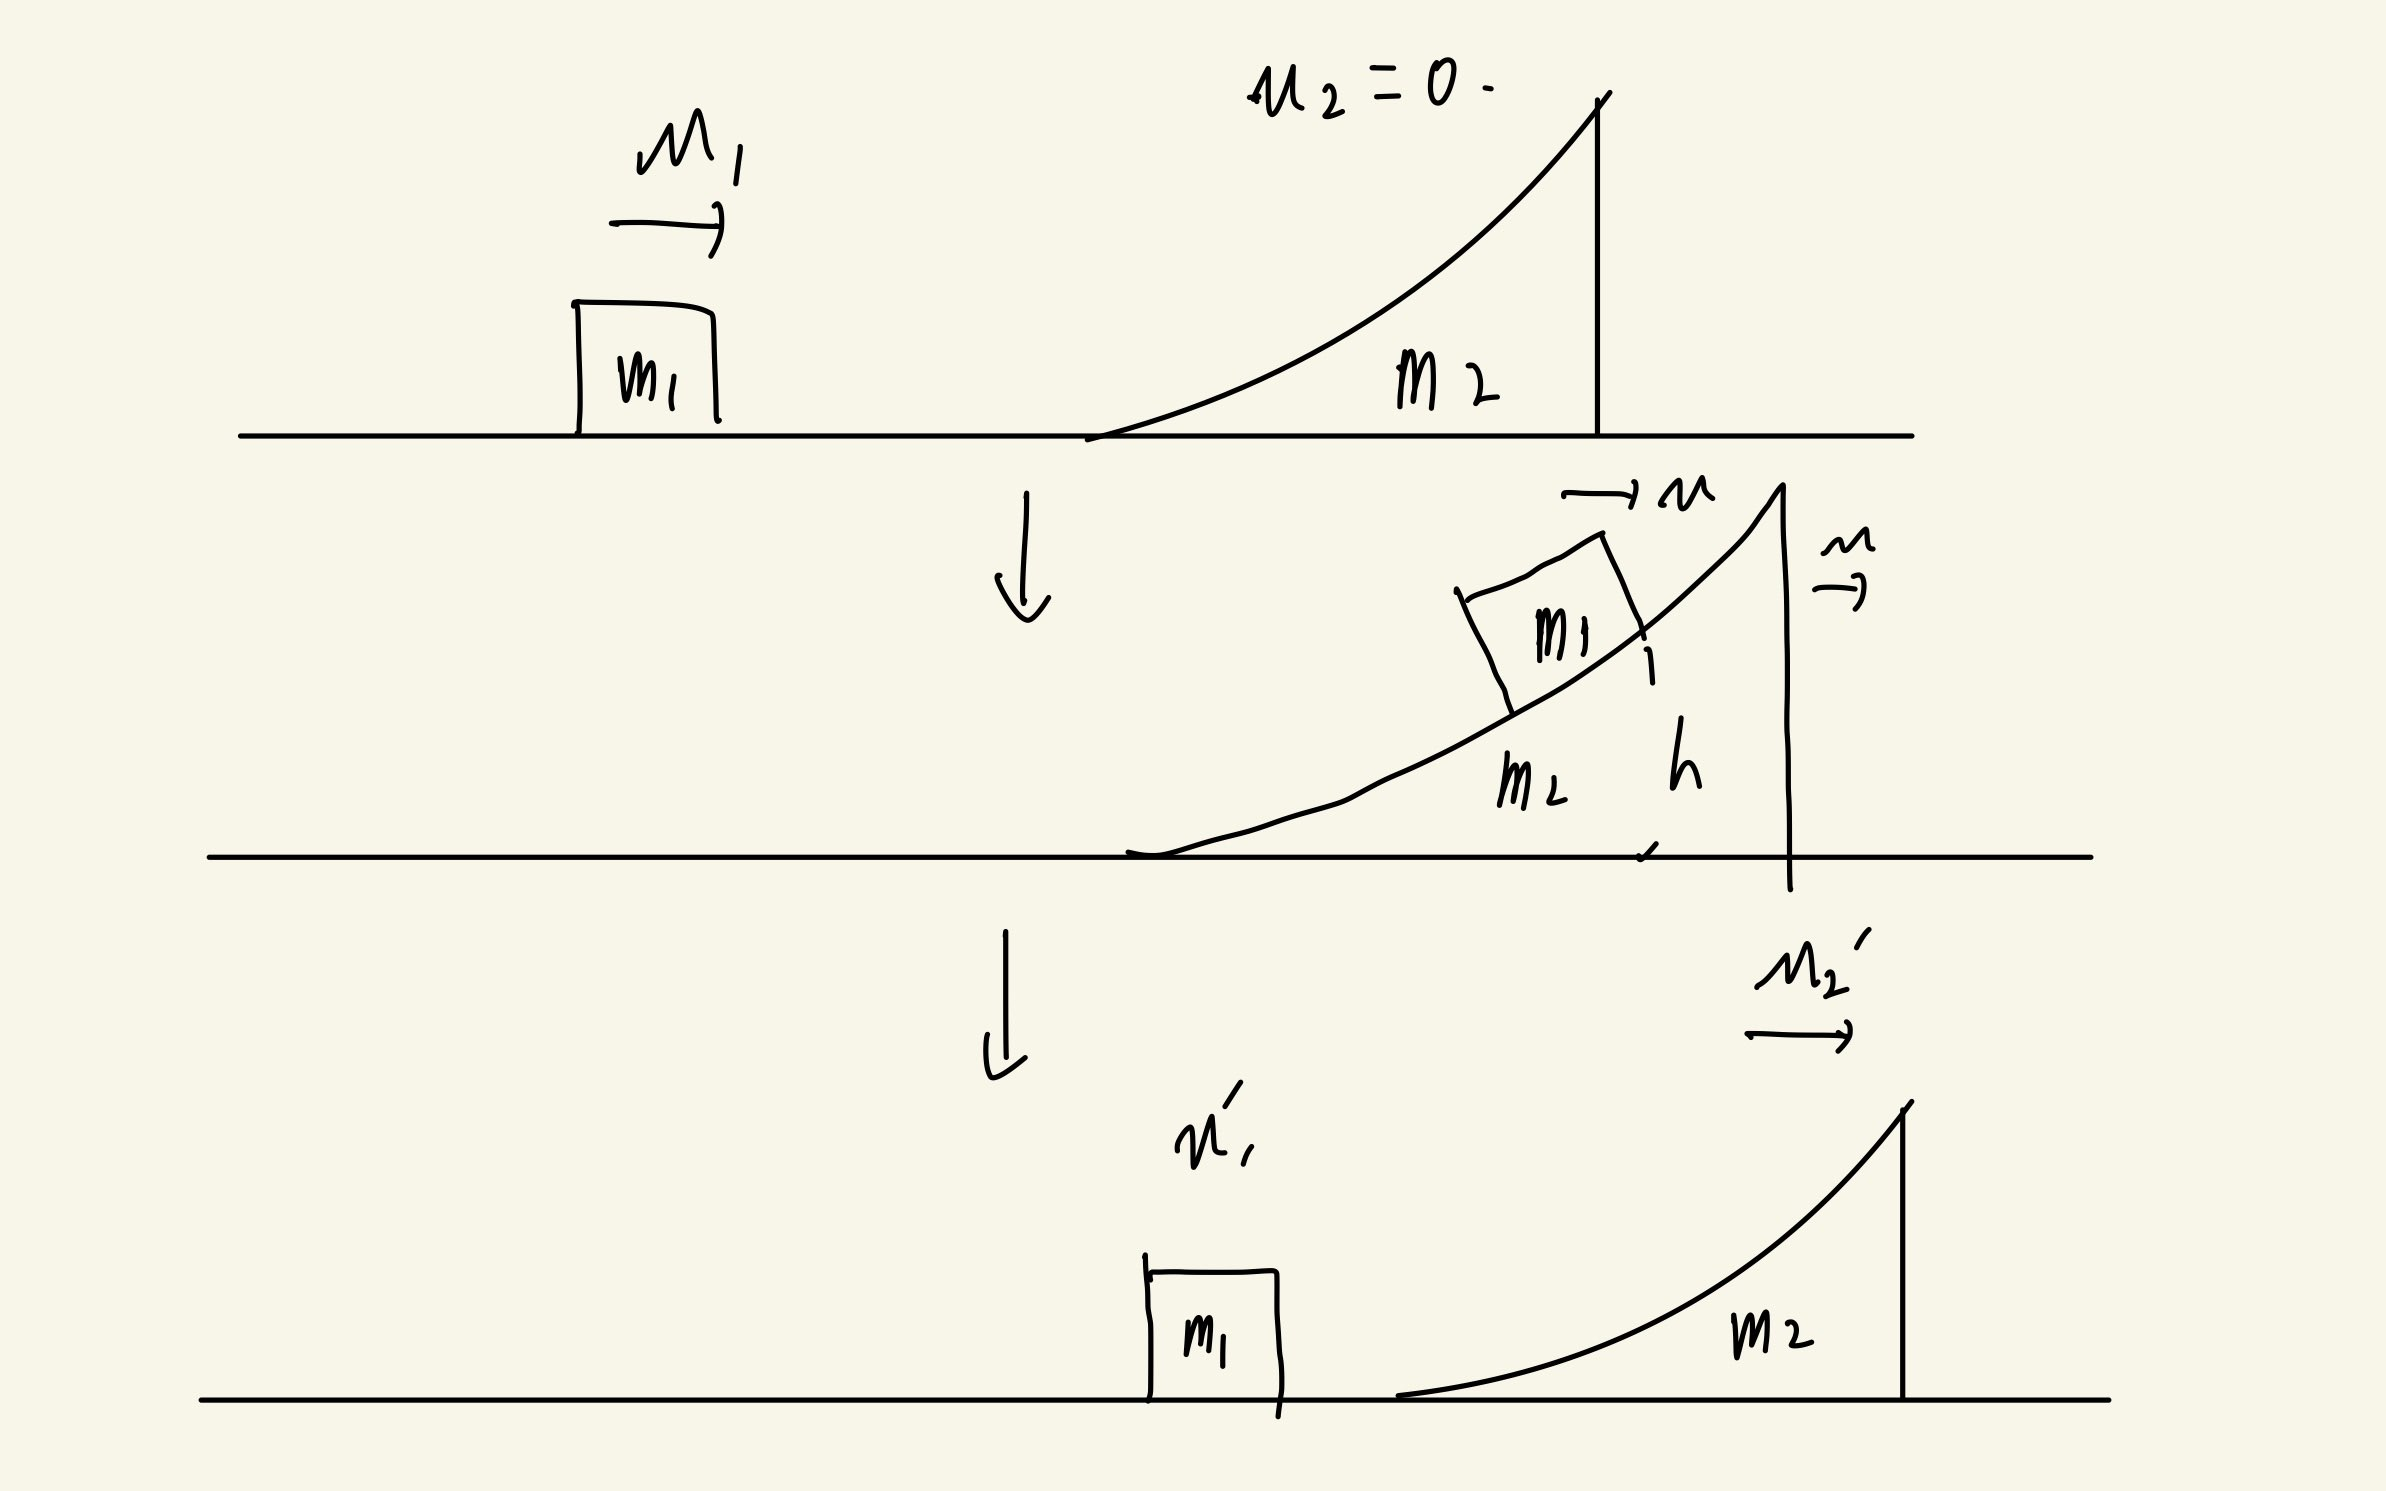
\includegraphics[width=100mm]{q.jpg}
    \end{center}
    \caption{問題の図}
    \label{fig:one}
\end{figure}
はじめ、物体1の速度は$v_1$であり、物体2の速度は0である。物体間の摩擦や床の摩擦、空気抵抗は無視できるものとする。
このとき、\\
(1) 物体1が物体2の最高点に到達したときの速度$v$を求めよ。\\
(2) 物体1が物体2の最高点に到達したときの物体1の地面からの高さを求めよ。\\
(3) 物体1が再び地面に到達したときの物体2の速度を求めよ。\\


\textbf{解答}\\
(1) 二体について水平方向の外力は加わっていないので、物体が最高点に到達したとき、その水平方向の速度は二体の重心速度に等しい。二体の最初の重心速度は、
\begin{align}
    v_{\text{g}} = \frac{m_1v_1}{m_1 + m_2}
\end{align}
であったから、これが求める速度である。\\
(2)力学的エネルギー保存則を考える。今、始めの状態と最高点の状態の運動エネルギーの差は、相対運動エネルギーの差に等しく、最高点において相対運動エネルギーが0であるから、
\begin{align}
    \Delta K = -\frac{1}{2}\mu v_1^2
\end{align}
である。(始めの相対速度が$v_1-0 = v_1$であることに注意)。ところで、この間に重力による仕事が$-m_1gh$だけなされる。したがって、
\begin{align}
    -m_1gh = -\frac{1}{2}\mu v_1^2
\end{align}
である。これを解いて、
\begin{align}
    h = \frac{\mu v_1^2}{2m_1g} = \frac{m_2v_1^2}{2(m_1 + m_2)g}
\end{align}
である。\\
(3) この問題は、反発係数1の衝突問題としてとらえることもできる。したがって、物体1が再び地面に到達したときの物体2の速度は、
\begin{align}
    v_2' &= -1\cdot(v_2 - v_{\text{g}}) +v_{\text{g}} \\
    &= -(0 - v_{\text{g}}) + v_{\text{g}} \\
    &= 2v_{\text{g}} \\
    &= \frac{2m_1v_1}{m_1 + m_2}
\end{align}
である。\\

おまけとして、物体1の最後の速度は、
\begin{align}
    v_1' = -(v_1 - v_{\text{g}}) + v_{\text{g}} = \frac{m_1-m_2}{m_1+m_2}v_1
\end{align}
である。\\


\end{document}